
% Default to the notebook output style

    


% Inherit from the specified cell style.




    
\documentclass[11pt]{article}

    
    
    \usepackage[T1]{fontenc}
    % Nicer default font (+ math font) than Computer Modern for most use cases
    \usepackage{mathpazo}

    % Basic figure setup, for now with no caption control since it's done
    % automatically by Pandoc (which extracts ![](path) syntax from Markdown).
    \usepackage{graphicx}
    % We will generate all images so they have a width \maxwidth. This means
    % that they will get their normal width if they fit onto the page, but
    % are scaled down if they would overflow the margins.
    \makeatletter
    \def\maxwidth{\ifdim\Gin@nat@width>\linewidth\linewidth
    \else\Gin@nat@width\fi}
    \makeatother
    \let\Oldincludegraphics\includegraphics
    % Set max figure width to be 80% of text width, for now hardcoded.
    \renewcommand{\includegraphics}[1]{\Oldincludegraphics[width=.8\maxwidth]{#1}}
    % Ensure that by default, figures have no caption (until we provide a
    % proper Figure object with a Caption API and a way to capture that
    % in the conversion process - todo).
    \usepackage{caption}
    \DeclareCaptionLabelFormat{nolabel}{}
    \captionsetup{labelformat=nolabel}

    \usepackage{adjustbox} % Used to constrain images to a maximum size 
    \usepackage{xcolor} % Allow colors to be defined
    \usepackage{enumerate} % Needed for markdown enumerations to work
    \usepackage{geometry} % Used to adjust the document margins
    \usepackage{amsmath} % Equations
    \usepackage{amssymb} % Equations
    \usepackage{textcomp} % defines textquotesingle
    % Hack from http://tex.stackexchange.com/a/47451/13684:
    \AtBeginDocument{%
        \def\PYZsq{\textquotesingle}% Upright quotes in Pygmentized code
    }
    \usepackage{upquote} % Upright quotes for verbatim code
    \usepackage{eurosym} % defines \euro
    \usepackage[mathletters]{ucs} % Extended unicode (utf-8) support
    \usepackage[utf8x]{inputenc} % Allow utf-8 characters in the tex document
    \usepackage{fancyvrb} % verbatim replacement that allows latex
    \usepackage{grffile} % extends the file name processing of package graphics 
                         % to support a larger range 
    % The hyperref package gives us a pdf with properly built
    % internal navigation ('pdf bookmarks' for the table of contents,
    % internal cross-reference links, web links for URLs, etc.)
    \usepackage{hyperref}
    \usepackage{longtable} % longtable support required by pandoc >1.10
    \usepackage{booktabs}  % table support for pandoc > 1.12.2
    \usepackage[inline]{enumitem} % IRkernel/repr support (it uses the enumerate* environment)
    \usepackage[normalem]{ulem} % ulem is needed to support strikethroughs (\sout)
                                % normalem makes italics be italics, not underlines
    

    
    
    % Colors for the hyperref package
    \definecolor{urlcolor}{rgb}{0,.145,.698}
    \definecolor{linkcolor}{rgb}{.71,0.21,0.01}
    \definecolor{citecolor}{rgb}{.12,.54,.11}

    % ANSI colors
    \definecolor{ansi-black}{HTML}{3E424D}
    \definecolor{ansi-black-intense}{HTML}{282C36}
    \definecolor{ansi-red}{HTML}{E75C58}
    \definecolor{ansi-red-intense}{HTML}{B22B31}
    \definecolor{ansi-green}{HTML}{00A250}
    \definecolor{ansi-green-intense}{HTML}{007427}
    \definecolor{ansi-yellow}{HTML}{DDB62B}
    \definecolor{ansi-yellow-intense}{HTML}{B27D12}
    \definecolor{ansi-blue}{HTML}{208FFB}
    \definecolor{ansi-blue-intense}{HTML}{0065CA}
    \definecolor{ansi-magenta}{HTML}{D160C4}
    \definecolor{ansi-magenta-intense}{HTML}{A03196}
    \definecolor{ansi-cyan}{HTML}{60C6C8}
    \definecolor{ansi-cyan-intense}{HTML}{258F8F}
    \definecolor{ansi-white}{HTML}{C5C1B4}
    \definecolor{ansi-white-intense}{HTML}{A1A6B2}

    % commands and environments needed by pandoc snippets
    % extracted from the output of `pandoc -s`
    \providecommand{\tightlist}{%
      \setlength{\itemsep}{0pt}\setlength{\parskip}{0pt}}
    \DefineVerbatimEnvironment{Highlighting}{Verbatim}{commandchars=\\\{\}}
    % Add ',fontsize=\small' for more characters per line
    \newenvironment{Shaded}{}{}
    \newcommand{\KeywordTok}[1]{\textcolor[rgb]{0.00,0.44,0.13}{\textbf{{#1}}}}
    \newcommand{\DataTypeTok}[1]{\textcolor[rgb]{0.56,0.13,0.00}{{#1}}}
    \newcommand{\DecValTok}[1]{\textcolor[rgb]{0.25,0.63,0.44}{{#1}}}
    \newcommand{\BaseNTok}[1]{\textcolor[rgb]{0.25,0.63,0.44}{{#1}}}
    \newcommand{\FloatTok}[1]{\textcolor[rgb]{0.25,0.63,0.44}{{#1}}}
    \newcommand{\CharTok}[1]{\textcolor[rgb]{0.25,0.44,0.63}{{#1}}}
    \newcommand{\StringTok}[1]{\textcolor[rgb]{0.25,0.44,0.63}{{#1}}}
    \newcommand{\CommentTok}[1]{\textcolor[rgb]{0.38,0.63,0.69}{\textit{{#1}}}}
    \newcommand{\OtherTok}[1]{\textcolor[rgb]{0.00,0.44,0.13}{{#1}}}
    \newcommand{\AlertTok}[1]{\textcolor[rgb]{1.00,0.00,0.00}{\textbf{{#1}}}}
    \newcommand{\FunctionTok}[1]{\textcolor[rgb]{0.02,0.16,0.49}{{#1}}}
    \newcommand{\RegionMarkerTok}[1]{{#1}}
    \newcommand{\ErrorTok}[1]{\textcolor[rgb]{1.00,0.00,0.00}{\textbf{{#1}}}}
    \newcommand{\NormalTok}[1]{{#1}}
    
    % Additional commands for more recent versions of Pandoc
    \newcommand{\ConstantTok}[1]{\textcolor[rgb]{0.53,0.00,0.00}{{#1}}}
    \newcommand{\SpecialCharTok}[1]{\textcolor[rgb]{0.25,0.44,0.63}{{#1}}}
    \newcommand{\VerbatimStringTok}[1]{\textcolor[rgb]{0.25,0.44,0.63}{{#1}}}
    \newcommand{\SpecialStringTok}[1]{\textcolor[rgb]{0.73,0.40,0.53}{{#1}}}
    \newcommand{\ImportTok}[1]{{#1}}
    \newcommand{\DocumentationTok}[1]{\textcolor[rgb]{0.73,0.13,0.13}{\textit{{#1}}}}
    \newcommand{\AnnotationTok}[1]{\textcolor[rgb]{0.38,0.63,0.69}{\textbf{\textit{{#1}}}}}
    \newcommand{\CommentVarTok}[1]{\textcolor[rgb]{0.38,0.63,0.69}{\textbf{\textit{{#1}}}}}
    \newcommand{\VariableTok}[1]{\textcolor[rgb]{0.10,0.09,0.49}{{#1}}}
    \newcommand{\ControlFlowTok}[1]{\textcolor[rgb]{0.00,0.44,0.13}{\textbf{{#1}}}}
    \newcommand{\OperatorTok}[1]{\textcolor[rgb]{0.40,0.40,0.40}{{#1}}}
    \newcommand{\BuiltInTok}[1]{{#1}}
    \newcommand{\ExtensionTok}[1]{{#1}}
    \newcommand{\PreprocessorTok}[1]{\textcolor[rgb]{0.74,0.48,0.00}{{#1}}}
    \newcommand{\AttributeTok}[1]{\textcolor[rgb]{0.49,0.56,0.16}{{#1}}}
    \newcommand{\InformationTok}[1]{\textcolor[rgb]{0.38,0.63,0.69}{\textbf{\textit{{#1}}}}}
    \newcommand{\WarningTok}[1]{\textcolor[rgb]{0.38,0.63,0.69}{\textbf{\textit{{#1}}}}}
    
    
    % Define a nice break command that doesn't care if a line doesn't already
    % exist.
    \def\br{\hspace*{\fill} \\* }
    % Math Jax compatability definitions
    \def\gt{>}
    \def\lt{<}
    % Document parameters
    \title{Exercise 1  Correlation Method}
    
    
    

    % Pygments definitions
    
\makeatletter
\def\PY@reset{\let\PY@it=\relax \let\PY@bf=\relax%
    \let\PY@ul=\relax \let\PY@tc=\relax%
    \let\PY@bc=\relax \let\PY@ff=\relax}
\def\PY@tok#1{\csname PY@tok@#1\endcsname}
\def\PY@toks#1+{\ifx\relax#1\empty\else%
    \PY@tok{#1}\expandafter\PY@toks\fi}
\def\PY@do#1{\PY@bc{\PY@tc{\PY@ul{%
    \PY@it{\PY@bf{\PY@ff{#1}}}}}}}
\def\PY#1#2{\PY@reset\PY@toks#1+\relax+\PY@do{#2}}

\expandafter\def\csname PY@tok@gd\endcsname{\def\PY@tc##1{\textcolor[rgb]{0.63,0.00,0.00}{##1}}}
\expandafter\def\csname PY@tok@gu\endcsname{\let\PY@bf=\textbf\def\PY@tc##1{\textcolor[rgb]{0.50,0.00,0.50}{##1}}}
\expandafter\def\csname PY@tok@gt\endcsname{\def\PY@tc##1{\textcolor[rgb]{0.00,0.27,0.87}{##1}}}
\expandafter\def\csname PY@tok@gs\endcsname{\let\PY@bf=\textbf}
\expandafter\def\csname PY@tok@gr\endcsname{\def\PY@tc##1{\textcolor[rgb]{1.00,0.00,0.00}{##1}}}
\expandafter\def\csname PY@tok@cm\endcsname{\let\PY@it=\textit\def\PY@tc##1{\textcolor[rgb]{0.25,0.50,0.50}{##1}}}
\expandafter\def\csname PY@tok@vg\endcsname{\def\PY@tc##1{\textcolor[rgb]{0.10,0.09,0.49}{##1}}}
\expandafter\def\csname PY@tok@vi\endcsname{\def\PY@tc##1{\textcolor[rgb]{0.10,0.09,0.49}{##1}}}
\expandafter\def\csname PY@tok@vm\endcsname{\def\PY@tc##1{\textcolor[rgb]{0.10,0.09,0.49}{##1}}}
\expandafter\def\csname PY@tok@mh\endcsname{\def\PY@tc##1{\textcolor[rgb]{0.40,0.40,0.40}{##1}}}
\expandafter\def\csname PY@tok@cs\endcsname{\let\PY@it=\textit\def\PY@tc##1{\textcolor[rgb]{0.25,0.50,0.50}{##1}}}
\expandafter\def\csname PY@tok@ge\endcsname{\let\PY@it=\textit}
\expandafter\def\csname PY@tok@vc\endcsname{\def\PY@tc##1{\textcolor[rgb]{0.10,0.09,0.49}{##1}}}
\expandafter\def\csname PY@tok@il\endcsname{\def\PY@tc##1{\textcolor[rgb]{0.40,0.40,0.40}{##1}}}
\expandafter\def\csname PY@tok@go\endcsname{\def\PY@tc##1{\textcolor[rgb]{0.53,0.53,0.53}{##1}}}
\expandafter\def\csname PY@tok@cp\endcsname{\def\PY@tc##1{\textcolor[rgb]{0.74,0.48,0.00}{##1}}}
\expandafter\def\csname PY@tok@gi\endcsname{\def\PY@tc##1{\textcolor[rgb]{0.00,0.63,0.00}{##1}}}
\expandafter\def\csname PY@tok@gh\endcsname{\let\PY@bf=\textbf\def\PY@tc##1{\textcolor[rgb]{0.00,0.00,0.50}{##1}}}
\expandafter\def\csname PY@tok@ni\endcsname{\let\PY@bf=\textbf\def\PY@tc##1{\textcolor[rgb]{0.60,0.60,0.60}{##1}}}
\expandafter\def\csname PY@tok@nl\endcsname{\def\PY@tc##1{\textcolor[rgb]{0.63,0.63,0.00}{##1}}}
\expandafter\def\csname PY@tok@nn\endcsname{\let\PY@bf=\textbf\def\PY@tc##1{\textcolor[rgb]{0.00,0.00,1.00}{##1}}}
\expandafter\def\csname PY@tok@no\endcsname{\def\PY@tc##1{\textcolor[rgb]{0.53,0.00,0.00}{##1}}}
\expandafter\def\csname PY@tok@na\endcsname{\def\PY@tc##1{\textcolor[rgb]{0.49,0.56,0.16}{##1}}}
\expandafter\def\csname PY@tok@nb\endcsname{\def\PY@tc##1{\textcolor[rgb]{0.00,0.50,0.00}{##1}}}
\expandafter\def\csname PY@tok@nc\endcsname{\let\PY@bf=\textbf\def\PY@tc##1{\textcolor[rgb]{0.00,0.00,1.00}{##1}}}
\expandafter\def\csname PY@tok@nd\endcsname{\def\PY@tc##1{\textcolor[rgb]{0.67,0.13,1.00}{##1}}}
\expandafter\def\csname PY@tok@ne\endcsname{\let\PY@bf=\textbf\def\PY@tc##1{\textcolor[rgb]{0.82,0.25,0.23}{##1}}}
\expandafter\def\csname PY@tok@nf\endcsname{\def\PY@tc##1{\textcolor[rgb]{0.00,0.00,1.00}{##1}}}
\expandafter\def\csname PY@tok@si\endcsname{\let\PY@bf=\textbf\def\PY@tc##1{\textcolor[rgb]{0.73,0.40,0.53}{##1}}}
\expandafter\def\csname PY@tok@s2\endcsname{\def\PY@tc##1{\textcolor[rgb]{0.73,0.13,0.13}{##1}}}
\expandafter\def\csname PY@tok@nt\endcsname{\let\PY@bf=\textbf\def\PY@tc##1{\textcolor[rgb]{0.00,0.50,0.00}{##1}}}
\expandafter\def\csname PY@tok@nv\endcsname{\def\PY@tc##1{\textcolor[rgb]{0.10,0.09,0.49}{##1}}}
\expandafter\def\csname PY@tok@s1\endcsname{\def\PY@tc##1{\textcolor[rgb]{0.73,0.13,0.13}{##1}}}
\expandafter\def\csname PY@tok@dl\endcsname{\def\PY@tc##1{\textcolor[rgb]{0.73,0.13,0.13}{##1}}}
\expandafter\def\csname PY@tok@ch\endcsname{\let\PY@it=\textit\def\PY@tc##1{\textcolor[rgb]{0.25,0.50,0.50}{##1}}}
\expandafter\def\csname PY@tok@m\endcsname{\def\PY@tc##1{\textcolor[rgb]{0.40,0.40,0.40}{##1}}}
\expandafter\def\csname PY@tok@gp\endcsname{\let\PY@bf=\textbf\def\PY@tc##1{\textcolor[rgb]{0.00,0.00,0.50}{##1}}}
\expandafter\def\csname PY@tok@sh\endcsname{\def\PY@tc##1{\textcolor[rgb]{0.73,0.13,0.13}{##1}}}
\expandafter\def\csname PY@tok@ow\endcsname{\let\PY@bf=\textbf\def\PY@tc##1{\textcolor[rgb]{0.67,0.13,1.00}{##1}}}
\expandafter\def\csname PY@tok@sx\endcsname{\def\PY@tc##1{\textcolor[rgb]{0.00,0.50,0.00}{##1}}}
\expandafter\def\csname PY@tok@bp\endcsname{\def\PY@tc##1{\textcolor[rgb]{0.00,0.50,0.00}{##1}}}
\expandafter\def\csname PY@tok@c1\endcsname{\let\PY@it=\textit\def\PY@tc##1{\textcolor[rgb]{0.25,0.50,0.50}{##1}}}
\expandafter\def\csname PY@tok@fm\endcsname{\def\PY@tc##1{\textcolor[rgb]{0.00,0.00,1.00}{##1}}}
\expandafter\def\csname PY@tok@o\endcsname{\def\PY@tc##1{\textcolor[rgb]{0.40,0.40,0.40}{##1}}}
\expandafter\def\csname PY@tok@kc\endcsname{\let\PY@bf=\textbf\def\PY@tc##1{\textcolor[rgb]{0.00,0.50,0.00}{##1}}}
\expandafter\def\csname PY@tok@c\endcsname{\let\PY@it=\textit\def\PY@tc##1{\textcolor[rgb]{0.25,0.50,0.50}{##1}}}
\expandafter\def\csname PY@tok@mf\endcsname{\def\PY@tc##1{\textcolor[rgb]{0.40,0.40,0.40}{##1}}}
\expandafter\def\csname PY@tok@err\endcsname{\def\PY@bc##1{\setlength{\fboxsep}{0pt}\fcolorbox[rgb]{1.00,0.00,0.00}{1,1,1}{\strut ##1}}}
\expandafter\def\csname PY@tok@mb\endcsname{\def\PY@tc##1{\textcolor[rgb]{0.40,0.40,0.40}{##1}}}
\expandafter\def\csname PY@tok@ss\endcsname{\def\PY@tc##1{\textcolor[rgb]{0.10,0.09,0.49}{##1}}}
\expandafter\def\csname PY@tok@sr\endcsname{\def\PY@tc##1{\textcolor[rgb]{0.73,0.40,0.53}{##1}}}
\expandafter\def\csname PY@tok@mo\endcsname{\def\PY@tc##1{\textcolor[rgb]{0.40,0.40,0.40}{##1}}}
\expandafter\def\csname PY@tok@kd\endcsname{\let\PY@bf=\textbf\def\PY@tc##1{\textcolor[rgb]{0.00,0.50,0.00}{##1}}}
\expandafter\def\csname PY@tok@mi\endcsname{\def\PY@tc##1{\textcolor[rgb]{0.40,0.40,0.40}{##1}}}
\expandafter\def\csname PY@tok@kn\endcsname{\let\PY@bf=\textbf\def\PY@tc##1{\textcolor[rgb]{0.00,0.50,0.00}{##1}}}
\expandafter\def\csname PY@tok@cpf\endcsname{\let\PY@it=\textit\def\PY@tc##1{\textcolor[rgb]{0.25,0.50,0.50}{##1}}}
\expandafter\def\csname PY@tok@kr\endcsname{\let\PY@bf=\textbf\def\PY@tc##1{\textcolor[rgb]{0.00,0.50,0.00}{##1}}}
\expandafter\def\csname PY@tok@s\endcsname{\def\PY@tc##1{\textcolor[rgb]{0.73,0.13,0.13}{##1}}}
\expandafter\def\csname PY@tok@kp\endcsname{\def\PY@tc##1{\textcolor[rgb]{0.00,0.50,0.00}{##1}}}
\expandafter\def\csname PY@tok@w\endcsname{\def\PY@tc##1{\textcolor[rgb]{0.73,0.73,0.73}{##1}}}
\expandafter\def\csname PY@tok@kt\endcsname{\def\PY@tc##1{\textcolor[rgb]{0.69,0.00,0.25}{##1}}}
\expandafter\def\csname PY@tok@sc\endcsname{\def\PY@tc##1{\textcolor[rgb]{0.73,0.13,0.13}{##1}}}
\expandafter\def\csname PY@tok@sb\endcsname{\def\PY@tc##1{\textcolor[rgb]{0.73,0.13,0.13}{##1}}}
\expandafter\def\csname PY@tok@sa\endcsname{\def\PY@tc##1{\textcolor[rgb]{0.73,0.13,0.13}{##1}}}
\expandafter\def\csname PY@tok@k\endcsname{\let\PY@bf=\textbf\def\PY@tc##1{\textcolor[rgb]{0.00,0.50,0.00}{##1}}}
\expandafter\def\csname PY@tok@se\endcsname{\let\PY@bf=\textbf\def\PY@tc##1{\textcolor[rgb]{0.73,0.40,0.13}{##1}}}
\expandafter\def\csname PY@tok@sd\endcsname{\let\PY@it=\textit\def\PY@tc##1{\textcolor[rgb]{0.73,0.13,0.13}{##1}}}

\def\PYZbs{\char`\\}
\def\PYZus{\char`\_}
\def\PYZob{\char`\{}
\def\PYZcb{\char`\}}
\def\PYZca{\char`\^}
\def\PYZam{\char`\&}
\def\PYZlt{\char`\<}
\def\PYZgt{\char`\>}
\def\PYZsh{\char`\#}
\def\PYZpc{\char`\%}
\def\PYZdl{\char`\$}
\def\PYZhy{\char`\-}
\def\PYZsq{\char`\'}
\def\PYZdq{\char`\"}
\def\PYZti{\char`\~}
% for compatibility with earlier versions
\def\PYZat{@}
\def\PYZlb{[}
\def\PYZrb{]}
\makeatother


    % Exact colors from NB
    \definecolor{incolor}{rgb}{0.0, 0.0, 0.5}
    \definecolor{outcolor}{rgb}{0.545, 0.0, 0.0}



    
    % Prevent overflowing lines due to hard-to-break entities
    \sloppy 
    % Setup hyperref package
    \hypersetup{
      breaklinks=true,  % so long urls are correctly broken across lines
      colorlinks=true,
      urlcolor=urlcolor,
      linkcolor=linkcolor,
      citecolor=citecolor,
      }
    % Slightly bigger margins than the latex defaults
    
    \geometry{verbose,tmargin=1in,bmargin=1in,lmargin=1in,rmargin=1in}
    
    

    \begin{document}
    
    
    \maketitle
    
    

    
    ** Xiangyi Cheng (xxc283)**

    \hypertarget{concepts-and-background}{%
\section{Concepts and Background}\label{concepts-and-background}}

    This notebook is created for explaining the basic idea of motion
estimation using correlation method. Motion estimation is the process of
determining motion vectors that describe the changing from one image to
another. The usage of motion estimation is highly critical and broad.
Tracking, detecting and identifying objects, computation of 3D structure
and position, object and scene segmentation are all the practical
applications related to motion estimation. Although the need and market
of the motion estimation is giant, motion estimation is still in
developing stage and there is no algorithm could ganrantee the high
accuracy in every motion. The good side is that there are various
algothrim are come up with by researchers in decades and it remains
interesting fields for us to dig deeper.

There are numerous motion estimation method such as block-matching
algorithm, phase correlation method, gradient method with solving motion
gradient constraint equation. This notebook is about to apply the
block-matching algorithm with correlation to estimate motion in two
images. The basic idea behind this algothrim is to split the first frame
into several blocks or grids. Then extract a patch from the previous
frame and set a larger area near this patch in the next frame called
search region as shown below. Correlations are calculated in each
location and check the biggest response in the computation. The maximum
response may be the same location in the next frame.
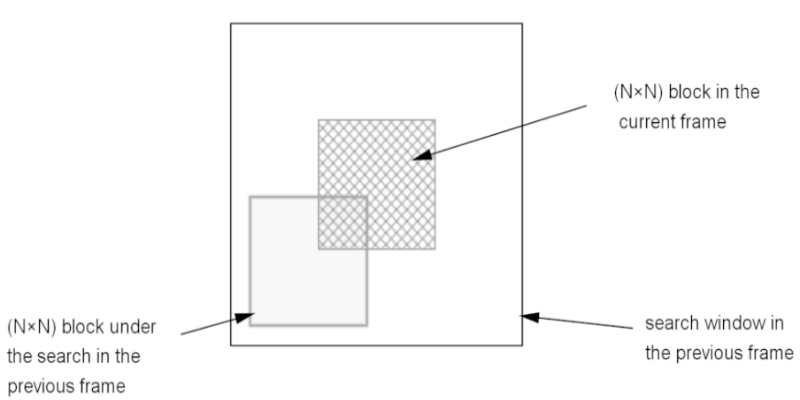
\includegraphics{block_r.png}

As for correlation, it is a useful concept in statistics. Correlation is
any of a broad class of statistical relationships and it most often
refers to how close two variables are to having a linear relationship
with each other. The population correlation coefficient ρX,Y between two
random variables X and Y with expected values μX and μY and standard
deviations σX and σY is defined as: 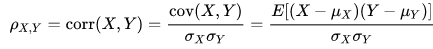
\includegraphics{cor.png}

If a series of n measurements of X and Y are obtained as xi and yi for i
= 1, 2, \ldots{}, n, then the sample correlation coefficient can be used
to estimate the population Pearson correlation r between X and Y. The
sample correlation coefficient is written as: 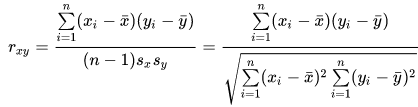
\includegraphics{cor1.png}

However, a build-in function to compute the correlation between two
matrix already exists in python so that the application is easier. With
the idea above, we can demonstrate the motion estimation in a simple
example as shown below.

    \hypertarget{implement}{%
\section{Implement}\label{implement}}

    To estimate the motion with correlation, several libraries are used and
imported.

    \begin{Verbatim}[commandchars=\\\{\}]
{\color{incolor}In [{\color{incolor}1}]:} \PY{k+kn}{from} \PY{n+nn}{scipy.signal} \PY{k+kn}{import} \PY{n}{correlate2d}
        \PY{k+kn}{import} \PY{n+nn}{numpy} \PY{k+kn}{as} \PY{n+nn}{np}
        \PY{k+kn}{import} \PY{n+nn}{matplotlib.pyplot} \PY{k+kn}{as} \PY{n+nn}{plt}
        \PY{k+kn}{from} \PY{n+nn}{skimage} \PY{k+kn}{import} \PY{n}{io}
\end{Verbatim}


    Read the image series into the computer. The first frame is named I1 and
the next frame is called I2.

    \begin{Verbatim}[commandchars=\\\{\}]
{\color{incolor}In [{\color{incolor}2}]:} \PY{n}{seq1} \PY{o}{=} \PY{p}{\PYZob{}}\PY{l+s+s1}{\PYZsq{}}\PY{l+s+s1}{I1}\PY{l+s+s1}{\PYZsq{}}\PY{p}{:} \PY{n}{io}\PY{o}{.}\PY{n}{imread}\PY{p}{(}\PY{l+s+s1}{\PYZsq{}}\PY{l+s+s1}{data/image/seq1/frame1.png}\PY{l+s+s1}{\PYZsq{}}\PY{p}{,} \PY{n}{as\PYZus{}grey}\PY{o}{=}\PY{n+nb+bp}{True}\PY{p}{)}\PY{p}{,} 
                \PY{l+s+s1}{\PYZsq{}}\PY{l+s+s1}{I2}\PY{l+s+s1}{\PYZsq{}}\PY{p}{:} \PY{n}{io}\PY{o}{.}\PY{n}{imread}\PY{p}{(}\PY{l+s+s1}{\PYZsq{}}\PY{l+s+s1}{data/image/seq1/frame3.png}\PY{l+s+s1}{\PYZsq{}}\PY{p}{,} \PY{n}{as\PYZus{}grey}\PY{o}{=}\PY{n+nb+bp}{True}\PY{p}{)}\PY{p}{,}
                \PY{l+s+s1}{\PYZsq{}}\PY{l+s+s1}{U}\PY{l+s+s1}{\PYZsq{}} \PY{p}{:} \PY{n}{np}\PY{o}{.}\PY{n}{loadtxt}\PY{p}{(}\PY{l+s+s1}{\PYZsq{}}\PY{l+s+s1}{data/flow/seq1/flow3.u}\PY{l+s+s1}{\PYZsq{}}\PY{p}{,} \PY{n}{dtype}\PY{o}{=}\PY{l+s+s1}{\PYZsq{}}\PY{l+s+s1}{double}\PY{l+s+s1}{\PYZsq{}}\PY{p}{,} \PY{n}{delimiter}\PY{o}{=}\PY{l+s+s1}{\PYZsq{}}\PY{l+s+s1}{,}\PY{l+s+s1}{\PYZsq{}}\PY{p}{)}\PY{p}{,}
                \PY{l+s+s1}{\PYZsq{}}\PY{l+s+s1}{V}\PY{l+s+s1}{\PYZsq{}} \PY{p}{:} \PY{n}{np}\PY{o}{.}\PY{n}{loadtxt}\PY{p}{(}\PY{l+s+s1}{\PYZsq{}}\PY{l+s+s1}{data/flow/seq1/flow3.v}\PY{l+s+s1}{\PYZsq{}}\PY{p}{,} \PY{n}{dtype}\PY{o}{=}\PY{l+s+s1}{\PYZsq{}}\PY{l+s+s1}{double}\PY{l+s+s1}{\PYZsq{}}\PY{p}{,} \PY{n}{delimiter}\PY{o}{=}\PY{l+s+s1}{\PYZsq{}}\PY{l+s+s1}{,}\PY{l+s+s1}{\PYZsq{}}\PY{p}{)}\PY{p}{\PYZcb{}}
        
        \PY{n}{rubic} \PY{o}{=} \PY{p}{\PYZob{}}\PY{l+s+s1}{\PYZsq{}}\PY{l+s+s1}{I1}\PY{l+s+s1}{\PYZsq{}}\PY{p}{:}\PY{n}{io}\PY{o}{.}\PY{n}{imread}\PY{p}{(}\PY{l+s+s1}{\PYZsq{}}\PY{l+s+s1}{data/rubic/rubic.0.png}\PY{l+s+s1}{\PYZsq{}}\PY{p}{,} \PY{n}{as\PYZus{}grey}\PY{o}{=}\PY{n+nb+bp}{True}\PY{p}{)}\PY{p}{,} 
                 \PY{l+s+s1}{\PYZsq{}}\PY{l+s+s1}{I2}\PY{l+s+s1}{\PYZsq{}}\PY{p}{:}\PY{n}{io}\PY{o}{.}\PY{n}{imread}\PY{p}{(}\PY{l+s+s1}{\PYZsq{}}\PY{l+s+s1}{data/rubic/rubic.5.png}\PY{l+s+s1}{\PYZsq{}}\PY{p}{,} \PY{n}{as\PYZus{}grey}\PY{o}{=}\PY{n+nb+bp}{True}\PY{p}{)}\PY{p}{\PYZcb{}}
        
        \PY{n}{sphere}\PY{o}{=} \PY{p}{\PYZob{}}\PY{l+s+s1}{\PYZsq{}}\PY{l+s+s1}{I1}\PY{l+s+s1}{\PYZsq{}}\PY{p}{:} \PY{n}{io}\PY{o}{.}\PY{n}{imread}\PY{p}{(}\PY{l+s+s1}{\PYZsq{}}\PY{l+s+s1}{data/sphere/sphere.1.png}\PY{l+s+s1}{\PYZsq{}}\PY{p}{,} \PY{n}{as\PYZus{}grey}\PY{o}{=}\PY{n+nb+bp}{True}\PY{p}{)}\PY{p}{,} 
                 \PY{l+s+s1}{\PYZsq{}}\PY{l+s+s1}{I2}\PY{l+s+s1}{\PYZsq{}}\PY{p}{:} \PY{n}{io}\PY{o}{.}\PY{n}{imread}\PY{p}{(}\PY{l+s+s1}{\PYZsq{}}\PY{l+s+s1}{data/sphere/sphere.3.png}\PY{l+s+s1}{\PYZsq{}}\PY{p}{,} \PY{n}{as\PYZus{}grey}\PY{o}{=}\PY{n+nb+bp}{True}\PY{p}{)}\PY{p}{\PYZcb{}}
\end{Verbatim}


    Define a function called correlation\_each\_grid() to extract the patch,
set the search region and calculate the correlation between two frames.
Firstly, some parameters such as image shape are given to the paramters.

Then the patch should be extracted from the first frame which is called
I1. Some conditions should be satisfied due to the image got the
boundaries and the patch cannot go beyond these boundaries.

The search region is based on the expand size and the patch with several
conditions as well.

Finally, the correlation is calculated using correlate2d(region, patch,
`valid') which is a build-in function for computing the corelation
between two matrices. The location of the maximum correlation is
obtained afterwards by np.unravel\_index(correlation.argmax(),
correlation.shape).

    \begin{Verbatim}[commandchars=\\\{\}]
{\color{incolor}In [{\color{incolor}7}]:} \PY{k}{def} \PY{n+nf}{correlation\PYZus{}each\PYZus{}grid}\PY{p}{(}\PY{n}{I1}\PY{p}{,} \PY{n}{I2}\PY{p}{,} \PY{n}{x}\PY{p}{,} \PY{n}{y}\PY{p}{,} \PY{n}{width}\PY{p}{,} \PY{n}{region\PYZus{}expand}\PY{p}{)}\PY{p}{:}
            \PY{n}{h}\PY{o}{=} \PY{n}{I1}\PY{o}{.}\PY{n}{shape}\PY{p}{[}\PY{l+m+mi}{0}\PY{p}{]}
            \PY{n}{w}\PY{o}{=} \PY{n}{I1}\PY{o}{.}\PY{n}{shape}\PY{p}{[}\PY{l+m+mi}{1}\PY{p}{]}
        
            \PY{n}{x} \PY{o}{=} \PY{n+nb}{int}\PY{p}{(}\PY{n}{x}\PY{p}{)}
            \PY{n}{y} \PY{o}{=} \PY{n+nb}{int}\PY{p}{(}\PY{n}{y}\PY{p}{)}
        
            \PY{n}{half\PYZus{}width} \PY{o}{=} \PY{n+nb}{int}\PY{p}{(}\PY{n}{np}\PY{o}{.}\PY{n}{floor}\PY{p}{(}\PY{n}{width}\PY{o}{/}\PY{l+m+mi}{2}\PY{p}{)}\PY{p}{)}
            
            
        \PY{c+c1}{\PYZsh{} patch construction}
            \PY{k}{if} \PY{p}{(}\PY{n}{y}\PY{o}{\PYZhy{}}\PY{n}{half\PYZus{}width}\PY{p}{)}\PY{o}{\PYZgt{}} \PY{l+m+mi}{0}\PY{p}{:}
                \PY{n}{p\PYZus{}x\PYZus{}up}\PY{o}{=}\PY{n}{y}\PY{o}{\PYZhy{}}\PY{n}{half\PYZus{}width}
            \PY{k}{else}\PY{p}{:}
                \PY{n}{p\PYZus{}x\PYZus{}up}\PY{o}{=}\PY{l+m+mi}{0}
        
            \PY{k}{if} \PY{p}{(}\PY{n}{y}\PY{o}{+}\PY{n}{half\PYZus{}width}\PY{o}{+}\PY{l+m+mi}{1}\PY{p}{)} \PY{o}{\PYZlt{}} \PY{n}{h}\PY{p}{:}
                \PY{n}{p\PYZus{}x\PYZus{}down}\PY{o}{=}\PY{n}{y}\PY{o}{+}\PY{n}{half\PYZus{}width}\PY{o}{+}\PY{l+m+mi}{1}
            \PY{k}{else}\PY{p}{:}
                \PY{n}{p\PYZus{}x\PYZus{}down}\PY{o}{=}\PY{n}{h}
        
            \PY{k}{if} \PY{p}{(}\PY{n}{x}\PY{o}{\PYZhy{}}\PY{n}{half\PYZus{}width}\PY{p}{)}\PY{o}{\PYZgt{}} \PY{l+m+mi}{0}\PY{p}{:}
                \PY{n}{p\PYZus{}y\PYZus{}left}\PY{o}{=}\PY{n}{x}\PY{o}{\PYZhy{}}\PY{n}{half\PYZus{}width}
            \PY{k}{else}\PY{p}{:}
                \PY{n}{p\PYZus{}y\PYZus{}left}\PY{o}{=}\PY{l+m+mi}{0}
        
            \PY{k}{if} \PY{p}{(}\PY{n}{x}\PY{o}{+}\PY{n}{half\PYZus{}width}\PY{o}{+}\PY{l+m+mi}{1}\PY{p}{)} \PY{o}{\PYZlt{}} \PY{n}{w}\PY{p}{:}
                \PY{n}{p\PYZus{}y\PYZus{}right}\PY{o}{=}\PY{n}{x}\PY{o}{+}\PY{n}{half\PYZus{}width}\PY{o}{+}\PY{l+m+mi}{1}
            \PY{k}{else}\PY{p}{:}
                \PY{n}{p\PYZus{}y\PYZus{}right}\PY{o}{=}\PY{n}{w}
        
            \PY{n}{patch} \PY{o}{=} \PY{n}{I1}\PY{p}{[}\PY{n}{p\PYZus{}x\PYZus{}up}\PY{p}{:}\PY{n}{p\PYZus{}x\PYZus{}down}\PY{p}{,} \PY{n}{p\PYZus{}y\PYZus{}left}\PY{p}{:}\PY{n}{p\PYZus{}y\PYZus{}right}\PY{p}{]}
            
            
            \PY{c+c1}{\PYZsh{} search region}
            \PY{k}{if} \PY{n}{y}\PY{o}{\PYZhy{}}\PY{n}{half\PYZus{}width}\PY{o}{\PYZhy{}}\PY{n}{region\PYZus{}expand}\PY{o}{\PYZgt{}} \PY{l+m+mi}{0}\PY{p}{:}
                \PY{n}{r\PYZus{}x\PYZus{}up}\PY{o}{=}\PY{n}{y}\PY{o}{\PYZhy{}}\PY{n}{half\PYZus{}width}\PY{o}{\PYZhy{}}\PY{n}{region\PYZus{}expand}
            \PY{k}{else}\PY{p}{:}
                \PY{n}{r\PYZus{}x\PYZus{}up}\PY{o}{=}\PY{l+m+mi}{0}
        
            \PY{k}{if} \PY{n}{y}\PY{o}{+}\PY{n}{half\PYZus{}width}\PY{o}{+}\PY{l+m+mi}{1}\PY{o}{+}\PY{n}{region\PYZus{}expand} \PY{o}{\PYZlt{}} \PY{n}{h}\PY{p}{:}
                \PY{n}{r\PYZus{}x\PYZus{}down}\PY{o}{=}\PY{n}{y}\PY{o}{+}\PY{n}{half\PYZus{}width}\PY{o}{+}\PY{l+m+mi}{1}\PY{o}{+}\PY{n}{region\PYZus{}expand}
            \PY{k}{else}\PY{p}{:}
                \PY{n}{r\PYZus{}x\PYZus{}down}\PY{o}{=}\PY{n}{h}
        
            \PY{k}{if} \PY{n}{x}\PY{o}{\PYZhy{}}\PY{n}{half\PYZus{}width}\PY{o}{\PYZhy{}}\PY{n}{region\PYZus{}expand} \PY{o}{\PYZgt{}} \PY{l+m+mi}{0}\PY{p}{:}
                \PY{n}{r\PYZus{}y\PYZus{}left} \PY{o}{=} \PY{n}{x}\PY{o}{\PYZhy{}}\PY{n}{half\PYZus{}width}\PY{o}{\PYZhy{}}\PY{n}{region\PYZus{}expand}
            \PY{k}{else}\PY{p}{:}
                \PY{n}{r\PYZus{}y\PYZus{}left}\PY{o}{=}\PY{l+m+mi}{0}
        
            \PY{k}{if} \PY{n}{x}\PY{o}{+}\PY{n}{half\PYZus{}width}\PY{o}{+}\PY{l+m+mi}{1}\PY{o}{+}\PY{n}{region\PYZus{}expand} \PY{o}{\PYZlt{}} \PY{n}{w}\PY{p}{:}
                \PY{n}{r\PYZus{}y\PYZus{}right}\PY{o}{=}\PY{n}{x}\PY{o}{+}\PY{n}{half\PYZus{}width}\PY{o}{+}\PY{l+m+mi}{1}\PY{o}{+}\PY{n}{region\PYZus{}expand}
            \PY{k}{else}\PY{p}{:}
                \PY{n}{r\PYZus{}y\PYZus{}right}\PY{o}{=}\PY{n}{w}
        
            \PY{n}{region} \PY{o}{=} \PY{n}{I2}\PY{p}{[}\PY{n}{r\PYZus{}x\PYZus{}up}\PY{p}{:}\PY{n}{r\PYZus{}x\PYZus{}down}\PY{p}{,} \PY{n}{r\PYZus{}y\PYZus{}left}\PY{p}{:}\PY{n}{r\PYZus{}y\PYZus{}right}\PY{p}{]}
            
            
            \PY{c+c1}{\PYZsh{} correlation}
            \PY{n}{correlation} \PY{o}{=} \PY{n}{correlate2d}\PY{p}{(}\PY{n}{region}\PY{p}{,} \PY{n}{patch}\PY{p}{,} \PY{l+s+s1}{\PYZsq{}}\PY{l+s+s1}{valid}\PY{l+s+s1}{\PYZsq{}}\PY{p}{)}
            \PY{n}{i}\PY{p}{,} \PY{n}{j} \PY{o}{=} \PY{n}{np}\PY{o}{.}\PY{n}{unravel\PYZus{}index}\PY{p}{(}\PY{n}{correlation}\PY{o}{.}\PY{n}{argmax}\PY{p}{(}\PY{p}{)}\PY{p}{,} \PY{n}{correlation}\PY{o}{.}\PY{n}{shape}\PY{p}{)}
            \PY{n}{u} \PY{o}{=} \PY{n}{j}\PY{o}{+}\PY{n}{r\PYZus{}y\PYZus{}left}\PY{o}{\PYZhy{}}\PY{n}{p\PYZus{}y\PYZus{}left}
            \PY{n}{v} \PY{o}{=} \PY{n}{i}\PY{o}{+}\PY{n}{r\PYZus{}x\PYZus{}up}\PY{o}{\PYZhy{}}\PY{n}{p\PYZus{}x\PYZus{}up}
        
            \PY{k}{return} \PY{p}{(}\PY{n}{u}\PY{p}{,} \PY{n}{v}\PY{p}{)}
\end{Verbatim}


    As shown above, the u and v matrices reflecting the motion is obtained
with this function. However, this is only for one block or grid not all
grids. Before solving that, to show the optical flow with quiver, a
function is defined to draw the vectors on the first frame with the
motion vectors to check the results.

    \begin{Verbatim}[commandchars=\\\{\}]
{\color{incolor}In [{\color{incolor}8}]:} \PY{k}{def} \PY{n+nf}{quiver\PYZus{}drawing}\PY{p}{(}\PY{n}{I}\PY{p}{,} \PY{n}{x\PYZus{}grid}\PY{p}{,} \PY{n}{y\PYZus{}grid}\PY{p}{,} \PY{n}{U}\PY{p}{,} \PY{n}{V}\PY{p}{,} \PY{n}{scale}\PY{p}{)}\PY{p}{:}
            \PY{n}{fig}\PY{p}{,} \PY{n}{ax} \PY{o}{=} \PY{n}{plt}\PY{o}{.}\PY{n}{subplots}\PY{p}{(}\PY{n}{figsize}\PY{o}{=}\PY{p}{(}\PY{l+m+mi}{10}\PY{p}{,} \PY{l+m+mi}{10}\PY{p}{)}\PY{p}{,} \PY{n}{dpi}\PY{o}{=}\PY{l+m+mi}{80}\PY{p}{)}
            \PY{n}{ax}\PY{o}{.}\PY{n}{imshow}\PY{p}{(}\PY{n}{I}\PY{p}{,} \PY{n}{cmap}\PY{o}{=}\PY{l+s+s1}{\PYZsq{}}\PY{l+s+s1}{gray}\PY{l+s+s1}{\PYZsq{}}\PY{p}{)}
            \PY{n}{ax}\PY{o}{.}\PY{n}{quiver}\PY{p}{(}\PY{n}{x\PYZus{}grid}\PY{p}{,} \PY{n}{y\PYZus{}grid}\PY{p}{,} \PY{n}{U}\PY{o}{*}\PY{n}{scale}\PY{p}{,} \PY{n}{V}\PY{o}{*}\PY{n}{scale}\PY{p}{,} \PY{n}{color}\PY{o}{=}\PY{l+s+s1}{\PYZsq{}}\PY{l+s+s1}{red}\PY{l+s+s1}{\PYZsq{}}\PY{p}{,} \PY{n}{angles}\PY{o}{=}\PY{l+s+s1}{\PYZsq{}}\PY{l+s+s1}{xy}\PY{l+s+s1}{\PYZsq{}}\PY{p}{,} \PY{n}{scale\PYZus{}units}\PY{o}{=}\PY{l+s+s1}{\PYZsq{}}\PY{l+s+s1}{xy}\PY{l+s+s1}{\PYZsq{}}\PY{p}{,} \PY{n}{scale}\PY{o}{=}\PY{l+m+mi}{1}\PY{p}{)}
            \PY{n}{ax}\PY{o}{.}\PY{n}{set\PYZus{}aspect}\PY{p}{(}\PY{l+s+s1}{\PYZsq{}}\PY{l+s+s1}{equal}\PY{l+s+s1}{\PYZsq{}}\PY{p}{)}
            \PY{n}{plt}\PY{o}{.}\PY{n}{show}\PY{p}{(}\PY{p}{)}
\end{Verbatim}


    A self-defined function is needed to calculate the motion vectors in
different grids. To achieve this goal, each grid is calculated and
filled in U and V matrices by iterations shown below.

quiver\_drawing() defined above is called to show the motion estimation
results which is also called optical flow.

    \begin{Verbatim}[commandchars=\\\{\}]
{\color{incolor}In [{\color{incolor}9}]:} \PY{k}{def} \PY{n+nf}{optical\PYZus{}flow\PYZus{}estimation}\PY{p}{(}\PY{n}{img\PYZus{}series}\PY{p}{)}\PY{p}{:}
            \PY{n}{h\PYZus{}img}\PY{o}{=} \PY{n}{img\PYZus{}series}\PY{p}{[}\PY{l+s+s1}{\PYZsq{}}\PY{l+s+s1}{I1}\PY{l+s+s1}{\PYZsq{}}\PY{p}{]}\PY{o}{.}\PY{n}{shape}\PY{p}{[}\PY{l+m+mi}{0}\PY{p}{]}
            \PY{n}{w\PYZus{}img}\PY{o}{=} \PY{n}{img\PYZus{}series}\PY{p}{[}\PY{l+s+s1}{\PYZsq{}}\PY{l+s+s1}{I1}\PY{l+s+s1}{\PYZsq{}}\PY{p}{]}\PY{o}{.}\PY{n}{shape}\PY{p}{[}\PY{l+m+mi}{1}\PY{p}{]}
        
            \PY{n}{grid\PYZus{}size} \PY{o}{=} \PY{l+m+mi}{5}
            \PY{n}{width}  \PY{o}{=} \PY{l+m+mi}{5}
        
            \PY{n}{x} \PY{o}{=} \PY{n}{np}\PY{o}{.}\PY{n}{arange}\PY{p}{(}\PY{l+m+mi}{0}\PY{p}{,} \PY{n}{w\PYZus{}img}\PY{o}{\PYZhy{}}\PY{n}{grid\PYZus{}size}\PY{p}{,} \PY{n}{grid\PYZus{}size}\PY{p}{)} \PY{o}{+} \PY{n}{np}\PY{o}{.}\PY{n}{floor}\PY{p}{(}\PY{n}{grid\PYZus{}size}\PY{o}{/}\PY{l+m+mi}{2}\PY{p}{)}\PY{p}{;}
            \PY{n}{y} \PY{o}{=} \PY{n}{np}\PY{o}{.}\PY{n}{arange}\PY{p}{(}\PY{l+m+mi}{0}\PY{p}{,} \PY{n}{h\PYZus{}img}\PY{o}{\PYZhy{}}\PY{n}{grid\PYZus{}size}\PY{p}{,} \PY{n}{grid\PYZus{}size}\PY{p}{)} \PY{o}{+} \PY{n}{np}\PY{o}{.}\PY{n}{floor}\PY{p}{(}\PY{n}{grid\PYZus{}size}\PY{o}{/}\PY{l+m+mi}{2}\PY{p}{)}\PY{p}{;}
            \PY{n}{x\PYZus{}grid}\PY{p}{,} \PY{n}{y\PYZus{}grid} \PY{o}{=} \PY{n}{np}\PY{o}{.}\PY{n}{meshgrid}\PY{p}{(}\PY{n}{x}\PY{p}{,}\PY{n}{y}\PY{p}{)}\PY{p}{;}
        
            \PY{n}{region\PYZus{}expand} \PY{o}{=} \PY{l+m+mi}{10}
        
            \PY{n}{h\PYZus{}grid} \PY{o}{=} \PY{n}{x\PYZus{}grid}\PY{o}{.}\PY{n}{shape}\PY{p}{[}\PY{l+m+mi}{0}\PY{p}{]}
            \PY{n}{w\PYZus{}grid} \PY{o}{=} \PY{n}{x\PYZus{}grid}\PY{o}{.}\PY{n}{shape}\PY{p}{[}\PY{l+m+mi}{1}\PY{p}{]}
        
            \PY{n}{U} \PY{o}{=} \PY{n}{np}\PY{o}{.}\PY{n}{zeros}\PY{p}{(}\PY{p}{(}\PY{n}{h\PYZus{}grid}\PY{p}{,} \PY{n}{w\PYZus{}grid}\PY{p}{)}\PY{p}{)}
            \PY{n}{V} \PY{o}{=} \PY{n}{np}\PY{o}{.}\PY{n}{zeros}\PY{p}{(}\PY{p}{(}\PY{n}{h\PYZus{}grid}\PY{p}{,} \PY{n}{w\PYZus{}grid}\PY{p}{)}\PY{p}{)}
            
            \PY{k}{for} \PY{n}{i} \PY{o+ow}{in} \PY{n+nb}{range}\PY{p}{(}\PY{l+m+mi}{0}\PY{p}{,} \PY{n}{h\PYZus{}grid}\PY{p}{)}\PY{p}{:}
                \PY{k}{for} \PY{n}{j} \PY{o+ow}{in} \PY{n+nb}{range}\PY{p}{(}\PY{l+m+mi}{0}\PY{p}{,} \PY{n}{w\PYZus{}grid}\PY{p}{)}\PY{p}{:}
                    \PY{n}{u}\PY{p}{,}\PY{n}{v} \PY{o}{=}  \PY{n}{correlation\PYZus{}each\PYZus{}grid}\PY{p}{(}\PY{n}{img\PYZus{}series}\PY{p}{[}\PY{l+s+s1}{\PYZsq{}}\PY{l+s+s1}{I1}\PY{l+s+s1}{\PYZsq{}}\PY{p}{]}\PY{p}{,} \PY{n}{img\PYZus{}series}\PY{p}{[}\PY{l+s+s1}{\PYZsq{}}\PY{l+s+s1}{I2}\PY{l+s+s1}{\PYZsq{}}\PY{p}{]}\PY{p}{,}
                                                 \PY{n}{x\PYZus{}grid}\PY{p}{[}\PY{n}{i}\PY{p}{,} \PY{n}{j}\PY{p}{]}\PY{p}{,} \PY{n}{y\PYZus{}grid}\PY{p}{[}\PY{n}{i}\PY{p}{,} \PY{n}{j}\PY{p}{]}\PY{p}{,} \PY{n}{width}\PY{p}{,} \PY{n}{region\PYZus{}expand}\PY{p}{)}
                    \PY{n}{U}\PY{p}{[}\PY{n}{i}\PY{p}{,} \PY{n}{j}\PY{p}{]} \PY{o}{=} \PY{n}{u}
                    \PY{n}{V}\PY{p}{[}\PY{n}{i}\PY{p}{,} \PY{n}{j}\PY{p}{]} \PY{o}{=} \PY{n}{v}
        
        
            \PY{n}{quiver\PYZus{}drawing}\PY{p}{(}\PY{n}{img\PYZus{}series}\PY{p}{[}\PY{l+s+s1}{\PYZsq{}}\PY{l+s+s1}{I1}\PY{l+s+s1}{\PYZsq{}}\PY{p}{]}\PY{p}{,}\PY{n}{x\PYZus{}grid}\PY{p}{,} \PY{n}{y\PYZus{}grid}\PY{p}{,} \PY{n}{U}\PY{p}{,} \PY{n}{V}\PY{p}{,} \PY{l+m+mi}{1}\PY{p}{)}
\end{Verbatim}


    Call the optical\_flow\_estimation() with different images and check the
result.

    \begin{Verbatim}[commandchars=\\\{\}]
{\color{incolor}In [{\color{incolor}10}]:} \PY{n}{optical\PYZus{}flow\PYZus{}estimation}\PY{p}{(}\PY{n}{sphere}\PY{p}{)}
\end{Verbatim}


    \begin{center}
    \adjustimage{max size={0.9\linewidth}{0.9\paperheight}}{output_15_0.png}
    \end{center}
    { \hspace*{\fill} \\}
    
    \begin{Verbatim}[commandchars=\\\{\}]
{\color{incolor}In [{\color{incolor}11}]:} \PY{n}{optical\PYZus{}flow\PYZus{}estimation}\PY{p}{(}\PY{n}{rubic}\PY{p}{)}
\end{Verbatim}


    \begin{center}
    \adjustimage{max size={0.9\linewidth}{0.9\paperheight}}{output_16_0.png}
    \end{center}
    { \hspace*{\fill} \\}
    
    \begin{Verbatim}[commandchars=\\\{\}]
{\color{incolor}In [{\color{incolor}12}]:} \PY{n}{optical\PYZus{}flow\PYZus{}estimation}\PY{p}{(}\PY{n}{seq1}\PY{p}{)}
\end{Verbatim}


    \begin{center}
    \adjustimage{max size={0.9\linewidth}{0.9\paperheight}}{output_17_0.png}
    \end{center}
    { \hspace*{\fill} \\}
    
    \hypertarget{exploration}{%
\section{Exploration}\label{exploration}}

    Another popular method in motion estimation similar to image corelation
is called \textbf{phase correlation}. Unlike the previous method with
calculating the correlation directly based on the image pixel, the phase
correlation method measures the movement between two frames from their
phases.

To calculate the phase correlation of the grids in respective frames,
FFT are first performed on the different frames. And the inverse FFT of
the multiplication of one spectrum and the conjugate of the other is
their phase correlation. The highest peak is picked out from the phase
corelation matrix to estimate the displacement vectors.

    To calculate the 2D FFT and inverse FFT, the functions are defined as
shown below.

    \begin{Verbatim}[commandchars=\\\{\}]
{\color{incolor}In [{\color{incolor}16}]:} \PY{k+kn}{from} \PY{n+nn}{scipy.fftpack} \PY{k+kn}{import} \PY{n}{dct}\PY{p}{,}\PY{n}{idct}
         \PY{k}{def} \PY{n+nf}{dct2}\PY{p}{(}\PY{n}{image}\PY{p}{)}\PY{p}{:}
             \PY{k}{return} \PY{n}{dct}\PY{p}{(}\PY{n}{dct}\PY{p}{(}\PY{n}{image}\PY{o}{.}\PY{n}{T}\PY{p}{,}\PY{n}{norm}\PY{o}{=}\PY{l+s+s1}{\PYZsq{}}\PY{l+s+s1}{ortho}\PY{l+s+s1}{\PYZsq{}}\PY{p}{)}\PY{o}{.}\PY{n}{T}\PY{p}{,}\PY{n}{norm}\PY{o}{=}\PY{l+s+s1}{\PYZsq{}}\PY{l+s+s1}{ortho}\PY{l+s+s1}{\PYZsq{}}\PY{p}{)}
         
         \PY{k}{def} \PY{n+nf}{idct2}\PY{p}{(}\PY{n}{dctmatrix}\PY{p}{)}\PY{p}{:}
             \PY{k}{return} \PY{n}{idct}\PY{p}{(}\PY{n}{idct}\PY{p}{(}\PY{n}{dctmatrix}\PY{o}{.}\PY{n}{T}\PY{p}{,}\PY{n}{norm}\PY{o}{=}\PY{l+s+s1}{\PYZsq{}}\PY{l+s+s1}{ortho}\PY{l+s+s1}{\PYZsq{}}\PY{p}{)}\PY{o}{.}\PY{n}{T}\PY{p}{,}\PY{n}{norm}\PY{o}{=}\PY{l+s+s1}{\PYZsq{}}\PY{l+s+s1}{ortho}\PY{l+s+s1}{\PYZsq{}}\PY{p}{)}
\end{Verbatim}


    Then redefine the correlation\_each\_grid() function to calculate the
correlation based on phase. Basically, apply FFT to the two frames, and
use the idea that the inverse FFT of the multiplication of one spectrum
and the conjugate of the other is their phase correlation to get the
correlation. Then check the highest response of the result.

    \begin{Verbatim}[commandchars=\\\{\}]
{\color{incolor}In [{\color{incolor}17}]:} \PY{k}{def} \PY{n+nf}{correlation\PYZus{}each\PYZus{}grid}\PY{p}{(}\PY{n}{I1}\PY{p}{,} \PY{n}{I2}\PY{p}{,} \PY{n}{x}\PY{p}{,} \PY{n}{y}\PY{p}{,} \PY{n}{width}\PY{p}{,} \PY{n}{region\PYZus{}expand}\PY{p}{)}\PY{p}{:}
             \PY{n}{h}\PY{o}{=} \PY{n}{I1}\PY{o}{.}\PY{n}{shape}\PY{p}{[}\PY{l+m+mi}{0}\PY{p}{]}
             \PY{n}{w}\PY{o}{=} \PY{n}{I1}\PY{o}{.}\PY{n}{shape}\PY{p}{[}\PY{l+m+mi}{1}\PY{p}{]}
         
             \PY{n}{x} \PY{o}{=} \PY{n+nb}{int}\PY{p}{(}\PY{n}{x}\PY{p}{)}
             \PY{n}{y} \PY{o}{=} \PY{n+nb}{int}\PY{p}{(}\PY{n}{y}\PY{p}{)}
         
             \PY{n}{half\PYZus{}width} \PY{o}{=} \PY{n+nb}{int}\PY{p}{(}\PY{n}{np}\PY{o}{.}\PY{n}{floor}\PY{p}{(}\PY{n}{width}\PY{o}{/}\PY{l+m+mi}{2}\PY{p}{)}\PY{p}{)}
         
             \PY{c+c1}{\PYZsh{} patch construction}
             \PY{k}{if} \PY{p}{(}\PY{n}{y}\PY{o}{\PYZhy{}}\PY{n}{half\PYZus{}width}\PY{p}{)}\PY{o}{\PYZgt{}} \PY{l+m+mi}{0}\PY{p}{:}
                 \PY{n}{p\PYZus{}x\PYZus{}up}\PY{o}{=}\PY{n}{y}\PY{o}{\PYZhy{}}\PY{n}{half\PYZus{}width}
             \PY{k}{else}\PY{p}{:}
                 \PY{n}{p\PYZus{}x\PYZus{}up}\PY{o}{=}\PY{l+m+mi}{0}
         
             \PY{k}{if} \PY{p}{(}\PY{n}{y}\PY{o}{+}\PY{n}{half\PYZus{}width}\PY{o}{+}\PY{l+m+mi}{1}\PY{p}{)} \PY{o}{\PYZlt{}} \PY{n}{h}\PY{p}{:}
                 \PY{n}{p\PYZus{}x\PYZus{}down}\PY{o}{=}\PY{n}{y}\PY{o}{+}\PY{n}{half\PYZus{}width}\PY{o}{+}\PY{l+m+mi}{1}
             \PY{k}{else}\PY{p}{:}
                 \PY{n}{p\PYZus{}x\PYZus{}down}\PY{o}{=}\PY{n}{h}
         
             \PY{k}{if} \PY{p}{(}\PY{n}{x}\PY{o}{\PYZhy{}}\PY{n}{half\PYZus{}width}\PY{p}{)}\PY{o}{\PYZgt{}} \PY{l+m+mi}{0}\PY{p}{:}
                 \PY{n}{p\PYZus{}y\PYZus{}left}\PY{o}{=}\PY{n}{x}\PY{o}{\PYZhy{}}\PY{n}{half\PYZus{}width}
             \PY{k}{else}\PY{p}{:}
                 \PY{n}{p\PYZus{}y\PYZus{}left}\PY{o}{=}\PY{l+m+mi}{0}
         
             \PY{k}{if} \PY{p}{(}\PY{n}{x}\PY{o}{+}\PY{n}{half\PYZus{}width}\PY{o}{+}\PY{l+m+mi}{1}\PY{p}{)} \PY{o}{\PYZlt{}} \PY{n}{w}\PY{p}{:}
                 \PY{n}{p\PYZus{}y\PYZus{}right}\PY{o}{=}\PY{n}{x}\PY{o}{+}\PY{n}{half\PYZus{}width}\PY{o}{+}\PY{l+m+mi}{1}
             \PY{k}{else}\PY{p}{:}
                 \PY{n}{p\PYZus{}y\PYZus{}right}\PY{o}{=}\PY{n}{w}
             
         
             \PY{n}{dct\PYZus{}img}\PY{o}{=}\PY{n}{dct2}\PY{p}{(}\PY{n}{I1}\PY{p}{)}
             \PY{n}{patch} \PY{o}{=} \PY{n}{dct\PYZus{}img}\PY{p}{[}\PY{n}{p\PYZus{}x\PYZus{}up}\PY{p}{:}\PY{n}{p\PYZus{}x\PYZus{}down}\PY{p}{,} \PY{n}{p\PYZus{}y\PYZus{}left}\PY{p}{:}\PY{n}{p\PYZus{}y\PYZus{}right}\PY{p}{]}
             
             \PY{c+c1}{\PYZsh{} correlation region}
             \PY{k}{if} \PY{n}{y}\PY{o}{\PYZhy{}}\PY{n}{half\PYZus{}width}\PY{o}{\PYZhy{}}\PY{n}{region\PYZus{}expand}\PY{o}{\PYZgt{}} \PY{l+m+mi}{0}\PY{p}{:}
                 \PY{n}{r\PYZus{}x\PYZus{}up}\PY{o}{=}\PY{n}{y}\PY{o}{\PYZhy{}}\PY{n}{half\PYZus{}width}\PY{o}{+}\PY{n}{region\PYZus{}expand}
             \PY{k}{else}\PY{p}{:}
                 \PY{n}{r\PYZus{}x\PYZus{}up}\PY{o}{=}\PY{l+m+mi}{0}
         
             \PY{k}{if} \PY{n}{y}\PY{o}{+}\PY{n}{half\PYZus{}width}\PY{o}{+}\PY{l+m+mi}{1}\PY{o}{+}\PY{n}{region\PYZus{}expand} \PY{o}{\PYZlt{}} \PY{n}{h}\PY{p}{:}
                 \PY{n}{r\PYZus{}x\PYZus{}down}\PY{o}{=}\PY{n}{y}\PY{o}{+}\PY{n}{half\PYZus{}width}\PY{o}{+}\PY{l+m+mi}{1}\PY{o}{+}\PY{n}{region\PYZus{}expand}
             \PY{k}{else}\PY{p}{:}
                 \PY{n}{r\PYZus{}x\PYZus{}down}\PY{o}{=}\PY{n}{h}
         
             \PY{k}{if} \PY{n}{x}\PY{o}{\PYZhy{}}\PY{n}{half\PYZus{}width}\PY{o}{\PYZhy{}}\PY{n}{region\PYZus{}expand} \PY{o}{\PYZgt{}} \PY{l+m+mi}{0}\PY{p}{:}
                 \PY{n}{r\PYZus{}y\PYZus{}left} \PY{o}{=} \PY{n}{x}\PY{o}{\PYZhy{}}\PY{n}{half\PYZus{}width}\PY{o}{+}\PY{n}{region\PYZus{}expand}
             \PY{k}{else}\PY{p}{:}
                 \PY{n}{r\PYZus{}y\PYZus{}left}\PY{o}{=}\PY{l+m+mi}{0}
         
             \PY{k}{if} \PY{n}{x}\PY{o}{+}\PY{n}{half\PYZus{}width}\PY{o}{+}\PY{l+m+mi}{1}\PY{o}{+}\PY{n}{region\PYZus{}expand} \PY{o}{\PYZlt{}} \PY{n}{w}\PY{p}{:}
                 \PY{n}{r\PYZus{}y\PYZus{}right}\PY{o}{=}\PY{n}{x}\PY{o}{+}\PY{n}{half\PYZus{}width}\PY{o}{+}\PY{l+m+mi}{1}\PY{o}{+}\PY{n}{region\PYZus{}expand}
             \PY{k}{else}\PY{p}{:}
                 \PY{n}{r\PYZus{}y\PYZus{}right}\PY{o}{=}\PY{n}{w}
         
             \PY{n}{dct\PYZus{}region}\PY{o}{=}\PY{n}{dct2}\PY{p}{(}\PY{n}{I2}\PY{p}{)}
             \PY{n}{region} \PY{o}{=} \PY{n}{dct\PYZus{}region}\PY{p}{[}\PY{n}{r\PYZus{}x\PYZus{}up}\PY{p}{:}\PY{n}{r\PYZus{}x\PYZus{}down}\PY{p}{,} \PY{n}{r\PYZus{}y\PYZus{}left}\PY{p}{:}\PY{n}{r\PYZus{}y\PYZus{}right}\PY{p}{]}
             
             \PY{c+c1}{\PYZsh{} correlation}
             \PY{c+c1}{\PYZsh{}correlation = correlate2d(region, patch, \PYZsq{}valid\PYZsq{})}
             \PY{n}{correlation}\PY{o}{=}\PY{n}{idct}\PY{p}{(}\PY{n}{patch}\PY{o}{*}\PY{n}{np}\PY{o}{.}\PY{n}{conjugate}\PY{p}{(}\PY{n}{region}\PY{p}{)}\PY{p}{)}
         
           
             \PY{n}{i}\PY{p}{,} \PY{n}{j} \PY{o}{=} \PY{n}{np}\PY{o}{.}\PY{n}{unravel\PYZus{}index}\PY{p}{(}\PY{n}{correlation}\PY{o}{.}\PY{n}{argmax}\PY{p}{(}\PY{p}{)}\PY{p}{,} \PY{n}{correlation}\PY{o}{.}\PY{n}{shape}\PY{p}{)}
             \PY{n}{u} \PY{o}{=} \PY{n}{j}\PY{o}{+}\PY{n}{r\PYZus{}y\PYZus{}left}\PY{o}{\PYZhy{}}\PY{n}{p\PYZus{}y\PYZus{}left}
             \PY{n}{v} \PY{o}{=} \PY{n}{i}\PY{o}{+}\PY{n}{r\PYZus{}x\PYZus{}up}\PY{o}{\PYZhy{}}\PY{n}{p\PYZus{}x\PYZus{}up}
         
             \PY{k}{return} \PY{p}{(}\PY{n}{u}\PY{p}{,} \PY{n}{v}\PY{p}{)}
\end{Verbatim}


    Make the region\_expand=0 to ensure patch and region have the same size
so that they can be multipiled.

    \begin{Verbatim}[commandchars=\\\{\}]
{\color{incolor}In [{\color{incolor}19}]:} \PY{k}{def} \PY{n+nf}{optical\PYZus{}flow\PYZus{}estimation}\PY{p}{(}\PY{n}{img\PYZus{}series}\PY{p}{)}\PY{p}{:}
             \PY{n}{h\PYZus{}img}\PY{o}{=} \PY{n}{img\PYZus{}series}\PY{p}{[}\PY{l+s+s1}{\PYZsq{}}\PY{l+s+s1}{I1}\PY{l+s+s1}{\PYZsq{}}\PY{p}{]}\PY{o}{.}\PY{n}{shape}\PY{p}{[}\PY{l+m+mi}{0}\PY{p}{]}
             \PY{n}{w\PYZus{}img}\PY{o}{=} \PY{n}{img\PYZus{}series}\PY{p}{[}\PY{l+s+s1}{\PYZsq{}}\PY{l+s+s1}{I1}\PY{l+s+s1}{\PYZsq{}}\PY{p}{]}\PY{o}{.}\PY{n}{shape}\PY{p}{[}\PY{l+m+mi}{1}\PY{p}{]}
         
             \PY{n}{grid\PYZus{}size} \PY{o}{=} \PY{l+m+mi}{10}
             \PY{n}{width}  \PY{o}{=} \PY{l+m+mi}{5}
         
             \PY{n}{x} \PY{o}{=} \PY{n}{np}\PY{o}{.}\PY{n}{arange}\PY{p}{(}\PY{l+m+mi}{0}\PY{p}{,} \PY{n}{w\PYZus{}img}\PY{o}{\PYZhy{}}\PY{n}{grid\PYZus{}size}\PY{p}{,} \PY{n}{grid\PYZus{}size}\PY{p}{)} \PY{o}{+} \PY{n}{np}\PY{o}{.}\PY{n}{floor}\PY{p}{(}\PY{n}{grid\PYZus{}size}\PY{o}{/}\PY{l+m+mi}{2}\PY{p}{)}\PY{p}{;}
             \PY{n}{y} \PY{o}{=} \PY{n}{np}\PY{o}{.}\PY{n}{arange}\PY{p}{(}\PY{l+m+mi}{0}\PY{p}{,} \PY{n}{h\PYZus{}img}\PY{o}{\PYZhy{}}\PY{n}{grid\PYZus{}size}\PY{p}{,} \PY{n}{grid\PYZus{}size}\PY{p}{)} \PY{o}{+} \PY{n}{np}\PY{o}{.}\PY{n}{floor}\PY{p}{(}\PY{n}{grid\PYZus{}size}\PY{o}{/}\PY{l+m+mi}{2}\PY{p}{)}\PY{p}{;}
             \PY{n}{x\PYZus{}grid}\PY{p}{,} \PY{n}{y\PYZus{}grid} \PY{o}{=} \PY{n}{np}\PY{o}{.}\PY{n}{meshgrid}\PY{p}{(}\PY{n}{x}\PY{p}{,}\PY{n}{y}\PY{p}{)}\PY{p}{;}
         
             \PY{n}{region\PYZus{}expand} \PY{o}{=} \PY{l+m+mi}{0}
         
             \PY{n}{h\PYZus{}grid} \PY{o}{=} \PY{n}{x\PYZus{}grid}\PY{o}{.}\PY{n}{shape}\PY{p}{[}\PY{l+m+mi}{0}\PY{p}{]}
             \PY{n}{w\PYZus{}grid} \PY{o}{=} \PY{n}{x\PYZus{}grid}\PY{o}{.}\PY{n}{shape}\PY{p}{[}\PY{l+m+mi}{1}\PY{p}{]}
         
             \PY{n}{U} \PY{o}{=} \PY{n}{np}\PY{o}{.}\PY{n}{zeros}\PY{p}{(}\PY{p}{(}\PY{n}{h\PYZus{}grid}\PY{p}{,} \PY{n}{w\PYZus{}grid}\PY{p}{)}\PY{p}{)}
             \PY{n}{V} \PY{o}{=} \PY{n}{np}\PY{o}{.}\PY{n}{zeros}\PY{p}{(}\PY{p}{(}\PY{n}{h\PYZus{}grid}\PY{p}{,} \PY{n}{w\PYZus{}grid}\PY{p}{)}\PY{p}{)}
             
             \PY{k}{for} \PY{n}{i} \PY{o+ow}{in} \PY{n+nb}{range}\PY{p}{(}\PY{l+m+mi}{0}\PY{p}{,} \PY{n}{h\PYZus{}grid}\PY{p}{)}\PY{p}{:}
                 \PY{k}{for} \PY{n}{j} \PY{o+ow}{in} \PY{n+nb}{range}\PY{p}{(}\PY{l+m+mi}{0}\PY{p}{,} \PY{n}{w\PYZus{}grid}\PY{p}{)}\PY{p}{:}
                     \PY{n}{u}\PY{p}{,}\PY{n}{v} \PY{o}{=}  \PY{n}{correlation\PYZus{}each\PYZus{}grid}\PY{p}{(}\PY{n}{img\PYZus{}series}\PY{p}{[}\PY{l+s+s1}{\PYZsq{}}\PY{l+s+s1}{I1}\PY{l+s+s1}{\PYZsq{}}\PY{p}{]}\PY{p}{,} 
                                                  \PY{n}{img\PYZus{}series}\PY{p}{[}\PY{l+s+s1}{\PYZsq{}}\PY{l+s+s1}{I2}\PY{l+s+s1}{\PYZsq{}}\PY{p}{]}\PY{p}{,}\PY{n}{x\PYZus{}grid}\PY{p}{[}\PY{n}{i}\PY{p}{,} \PY{n}{j}\PY{p}{]}\PY{p}{,} \PY{n}{y\PYZus{}grid}\PY{p}{[}\PY{n}{i}\PY{p}{,} \PY{n}{j}\PY{p}{]}\PY{p}{,} \PY{n}{width}\PY{p}{,} \PY{n}{region\PYZus{}expand}\PY{p}{)}
                     \PY{n}{U}\PY{p}{[}\PY{n}{i}\PY{p}{,} \PY{n}{j}\PY{p}{]} \PY{o}{=} \PY{n}{u}
                     \PY{n}{V}\PY{p}{[}\PY{n}{i}\PY{p}{,} \PY{n}{j}\PY{p}{]} \PY{o}{=} \PY{n}{v}
         
         
             \PY{n}{quiver\PYZus{}drawing}\PY{p}{(}\PY{n}{img\PYZus{}series}\PY{p}{[}\PY{l+s+s1}{\PYZsq{}}\PY{l+s+s1}{I1}\PY{l+s+s1}{\PYZsq{}}\PY{p}{]}\PY{p}{,}\PY{n}{x\PYZus{}grid}\PY{p}{,} \PY{n}{y\PYZus{}grid}\PY{p}{,} \PY{n}{U}\PY{p}{,} \PY{n}{V}\PY{p}{,} \PY{l+m+mi}{1}\PY{p}{)}
\end{Verbatim}


    Check the results.

    \begin{Verbatim}[commandchars=\\\{\}]
{\color{incolor}In [{\color{incolor}20}]:} \PY{n}{optical\PYZus{}flow\PYZus{}estimation}\PY{p}{(}\PY{n}{sphere}\PY{p}{)}
\end{Verbatim}


    \begin{center}
    \adjustimage{max size={0.9\linewidth}{0.9\paperheight}}{output_27_0.png}
    \end{center}
    { \hspace*{\fill} \\}
    
    The result seems not really reasonable. However, in one paper called
``Phase- Correlation Motion Estimation'' written by Yi Liang, the result
is robuster than the image correlation. An example he post is to compare
these two methods by estimating the bus motion as shown below.

\begin{figure}
\centering
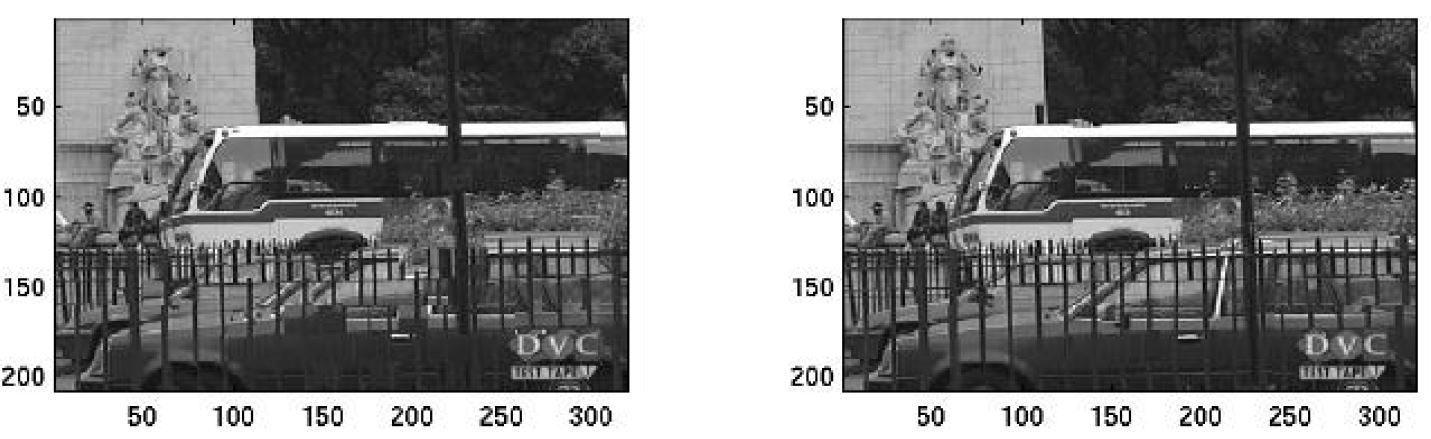
\includegraphics{ex2.jpg}
\caption{caption}
\end{figure}

\begin{figure}
\centering
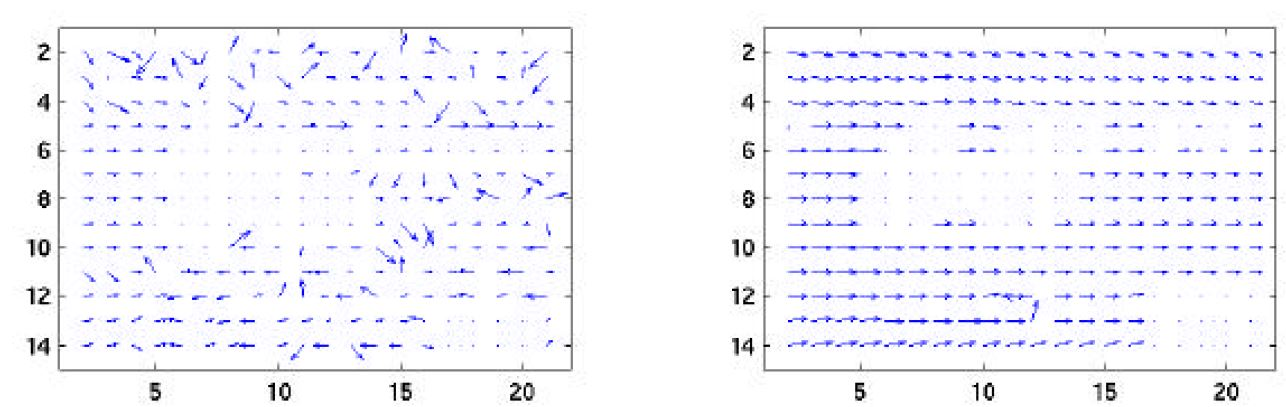
\includegraphics{ex.jpg}
\caption{caption}
\end{figure}

    \hypertarget{conclusion-and-discussion}{%
\section{Conclusion and Discussion}\label{conclusion-and-discussion}}

    From the results shown above, we can tell that the correlation method is
not reliable in some cases. The optical flow is relatively messy
compared to gradient method which will be explained in exercise 2. And
the application with phase correlation is not matching the reality as
well. After changing the grid in the code, I found that grid size
greatly affects the performances.

However, for the bus example within paper ``Phase- Correlation Motion
Estimation'', it demonstrates that phase correlation works better than
the image correlation does in the cases of large scale translation
motion. Moreover, phase correlation is computationally efficient and it
produces much smoother motion field.

    \hypertarget{reference}{%
\section{Reference}\label{reference}}

    https://en.wikipedia.org/wiki/Motion\_estimation

https://en.wikipedia.org/wiki/Block-matching\_algorithm

https://en.wikipedia.org/wiki/Correlation\_and\_dependence

Yi Liang, ``Phase- Correlation Motion Estimation'', EE392J Final
Project, Stanford University.


    % Add a bibliography block to the postdoc
    
    
    
    \end{document}
